\documentclass[12pt]{article}
\usepackage{sbc-template}
\usepackage{url}
\usepackage{graphicx}
\usepackage{paralist}
\usepackage{epstopdf}
%\usepackage[pdftex]{graphicx}
\usepackage{longtable}
\usepackage[utf8]{inputenc}
\usepackage{scalefnt}
\usepackage{easylist}
\usepackage{multirow}
\usepackage{float}
\usepackage[section]{placeins}
\usepackage{paralist}
\usepackage[final]{pdfpages}
\usepackage[brazilian]{babel}
\usepackage{cite}
\def\UrlFont{\tt\scriptsize}

\sloppy

\title{Aferição da Qualidade do Código-Fonte com apoio de um ambiente de \textit{Data Warehousing} na gestão de contrato ágil: um estudo de caso preliminar em uma autarquia da Administração Pública Federal}
\author{Guilherme Baufaker Rêgo$^1$, Hilmer Rodrigues Neri$^1$, Aline Gonçalves do Santos$^1$}
\address{Faculdade UnB Gama -- Universidade de Brasília
\email{hilmer@unb.br, gbre.111@gmail.com, alinegsantoss@gmail.com}
}

\begin{document}


\maketitle
\begin{abstract}

Some organizations of Federal Brazilian Goverment have started to use agile methods on software development contracts. In that situation, it have been observed the opportunity to enhance public organizations on measuring the internal quality of software outsourced. This work objective was propose an automated solution, based on data warehousing enviroment, which could measure the quality of source code in order to approve or reject by contractor. In order to get a empirical working evidence of that automated solution, it had been taken a place a case study where evaluated the 24 monthly realeases of Sistema Integrado de Gestão e Conhecimento (SIGC) from IPHAN, which it has meant more than 39.000 source code lines evaluated.

\end{abstract}
% Seção do Resumo
\begin{resumo}

Atualmente, algumas organizações da Administração Pública Federal iniciam investimentos para adotar contratações de serviços de desenvolvimento de \textit{software} utilizando métodos ágeis. Nestes processos de contratação percebeu-se a lacuna de como incorporar a qualidade interna do produto recebido como um critério de aceitação. O objetivo deste trabalho foi propor uma solução automatizada, apoiada em um ambiente de \textit{data warehousing}, que pudesse aferir elementos do código-fonte de forma a apoiar a aceitação ou rejeição do produto por parte da contrante. Visando a validação empírica da solução automatizada, realizou-se um estudo de caso no qual foi avaliado as 24 releases mensais do Sistema Integrado de Gestão e Conhecimento (SIGC) do IPHAN no qual foram avaliadas mais de 39.000 linhas de código-fonte. 

\end{resumo}

% Seção da Introdução
\section{Introdução}
\label{intro}

No desenvolvimento de software, há diversas variáveis, quer sejam de natureza ambiental ou técnica, que provavelmente impactarão desde a execução do processo de análise de requisitos até a implantação do software \cite{beckarticle1999}. Essa característica torna o processo de desenvolvimento pouco previsível e complexo, requerendo flexibilidade e personalização para ser capaz de responder às mudanças. 
Em consonância a esse movimento, órgãos da Administração Pública Federal (APF) também têm aderido a utilização de metodologias ágeis nos processos de desenvolvimento de software.

Recentemente, Tribunal de Contas da União publicou o Acórdão no 2314/2013 \cite{TCU:2013}
com práticas de contratação realizadas por instituições públicas federais, como por exemplo, Banco Central do Brasil (BACEN), Instituto do Patrimônio Histórico e Artístico Nacional (IPHAN), Instituto Nacional de Estudos e Pesquisas Educacionais Anísio Texeira (INEP), Tribunal Superior do Trabalho (TST) e Supremo Tribunal Federal (STF). Nestes órgãos, alguns casos de sucesso advém de processos de desenvolvimento interno e também por meio da transferência da execução tarefas executivas não ligadas com a função fim para iniciativa privada na prática conhecida comumente como terceirização de serviços que é apoiada pela legislação brasileira na Lei 8.666/1993 \cite{Lei8666:1993} que estabelece normas gerais sobre licitações e contratos administrativos; no Decreto-Lei 200/1967 que enunciou sobre a execução indireta de funções não finalísticas visando impedir o crescimento desmesurado da máquina administrativa e na Instrução Normativa nº 4 \cite{IN04:2010} que versa sobre o processo de Contratação de Soluções de Tecnologia da Informação pelos órgãos integrantes do Sistema de Administração dos Recursos de Informação e Informática do Poder Executivo Federal.

A Instrução Normativa nº 4 \cite{IN04:2010}, que é a norma mais recente, enuncia um conjunto e boas práticas e um modelo processo de contratações conforme visto na figura \ref{processo}. 

\begin{figure}[h]
        \centering
        \label{processo}
            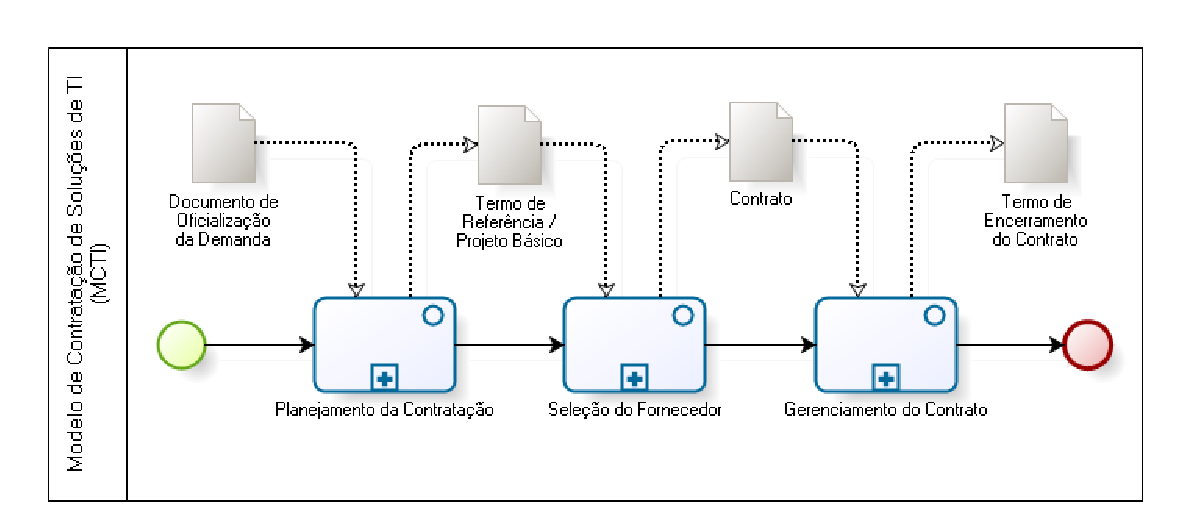
\includegraphics[scale=0.7]{figuras/MCTI.eps}
        \caption{Modelo de Processo de Contratações de Soluções de TI \cite{mcti}}
\end{figure}

A fase de Gerenciamento do Contrato visa acompanhar e garantir a adequada prestação do serviço e o fornecimento de bens que compõem a solução de TI, sendo que está disposto no art. 25 III, alínea b), que a avaliação da qualidade dos serviços realizados ou dos bens entregues e justificativas deve estar de acordo com os Critérios de Aceitação definidos em contrato, a cargo dos Fiscais Técnico e Requisitante do Contrato \cite{IN04:2010}.

Considerando o princípio ágil de valoração de produto sobre documentação abrangente, com objetivo de melhorar a qualidade interna utilizando de práticas do eXtreme Programmming, como por exemplo, desenvolvimento orientado a testes, refatoração e integração contínua do código-fonte \cite{beck1999} e que alínea b) do art 25 da IN04 especifica a necessidade da criação de critérios de aceitação, foi elaborada a seguinte questão de pesquisa: 

\textbf{Como incorporar, do ponto de vista do fiscal técnico do contrato, a qualidade do código-fonte como critério de aceitabilidade do produto?} 

A partir da questão de pesquisa, foram elaborados objetivos específicos utilizando o GQM \cite{Basili96b}. Nesta abordagem cada objetivo específico derivou uma série de questões específicas que são respondidas com métricas específicas, tal como se mostra na Tabela \ref{tbl:obj}

\begin{table}[ht]
\centering
\input{tabelas/objetivos.ltx}
\caption{Objetivos Específicos do Trabalho}
\label{tbl:obj} 
\end{table}
\FloatBarrier
% Seção de Métricas e Cenários de Limpeza de Código-Fonte
\section{Medição da Qualidade Interna do Produto}

A qualidade interna do produto de software pode ser medida, ainda em ambiente de desenvolvimento, por meio da avaliação de estruturas internas que compõem o sistema de software \cite{ISO25023}, sendo que as métricas extraídas diretamente do código-fonte são bons indicadores de qualidade interna de produto \cite{beck2003test}, pois são métricas objetivas e com características como validade, simplicidade, objetividade, fácil obtenção e robustez \cite{Mills:1999}.  


Para a escolha das métricas utilizadas neste trabalho, consideramos: i) os estudos encontrados na literatura sobre métricas de código-fonte, entre eles o trabalho de Marinescu \cite{marinescu2005measurement} um dos mais reconhecidos nesta área; ii) a existência de estudos que definem valores de referência para análise das métricas dos conceitos mais relevantes à manutenibilidade do software como o tamanho, complexidade interna, modularidade e grau de depedência entre módulos \cite{Meirelles2013}; iii) métricas que reflitam indicadores sobre boas práticas de programação, a exemplo da aderência a padrões de projeto e boas práticas de programação \cite{Machini2010}; iv) a existência das métricas na ferramenta de análise estática de código-fonte utilizada neste trabalho. Essas métricas escolhidas foram reunidas e são apresentadas na Tabela \ref{orientacao}.     


	\begin{table}[!h]
	\caption{Conjunto de Métricas de Código-Fonte}
	\addtolength{\belowcaptionskip}{6pt}
	\begin{center}
	\input{tabelas/orientacao-objeto.ltx}
	\label{orientacao}
	\end{center}
	\end{table}


Em um trabalho recente sobre a análise de métricas de código-fonte, foi observado o comportamento estatístico das métricas de código-fonte de 38 projetos de software livre com mais de 100.000 downloads em um esforço de análise de mais de 300.000 classes. Entre os softwares analisados estão Tomcat, OpenJDK, Eclipse, Google Chrome, VLC e outros que foram desenvolvidos em C, C++ e Java \cite{Meirelles2013}. Neste trabalho, concluiu-se empiricamente que há valores de referência para métricas de código-fonte, que foram classificados como muito frequentes, frequentes, pouco frequentes e não frequentes para softwares escritos em uma mesma linguagem de programação. Nos trabalhos como os de Marinescu \cite{marinescu2005measurement}, Moha \cite{moha2010decor} e Rao \cite{rao2007detecting}, foi mostrado que é possível utilizar métricas de código-fonte como forma de detecção de trechos de código-fonte que podem ser melhorados com a refatoração \cite{fowler1999refactoring}. Seguindo a abordagem de Marinescu, Machini \cite{Machini2010} mapeou as técnicas e práticas de limpeza de código-fonte propostas por \cite{Martin2008} e \cite{beck2007implementation} de forma a constuir cenários de limpeza de código-fonte que são recomendações ou práticas para eliminar um determinado trecho de código-fonte não coeso. No trabalho de \cite{Machini2010}, não foi utilizada nenhuma automatização para cálculo das métricas e posterior identificação de um cenário de limpeza.

De posse da análise estatística efetuada por Meirelles \cite{Meirelles2013}, agregamos as configurações dos intervalos de métricas como a forma de detecção dos cenários de limpeza propostos por \cite{Machini2010}, tal como se é possível observar na Tabela \ref{tab:cenarios}.
	
	\begin{table}[ht]
	\centering
	\caption{Detecção dos Cenários de Limpeza de Código-Fonte}
	\addtolength{\belowcaptionskip}{6pt}
	\input{tabelas/cenarios.ltx}	
	\label{tab:cenarios}
	\end{table}
	\FloatBarrier


A partir da identificação dos cenários de limpeza de código-fonte e da contagem do número de classes em uma determinada \textit{release} do software, criamos a Taxa de Aproveitamento de Oportunidade de Melhoria de Código-Fonte $(T_r)$ como um indicador objetivo de monitoramento da oportunidade de melhoria da qualidade do código-fonte, sendo este descrito conforme a Equação \ref{eqn01}, em que $ Ce_r $ é o total de cenários de limpeza na release e $ Cl_r $ é a quantidade classes na mesma release.

\begin{equation}
\label{eqn01}
T_r =   \frac{{{Ce_r}}}{{Cl_r}}
\end{equation}

% Seção da Solução com o Uso de DW
\section{Solução para Automação do Processo de Medição da Qualidade Interna do Produto}
\label{sec:solucao}

Visando atingir a automação do processo de medição de qualidade interna do produto por meio de técnicas não intrusivas no ambiente de desenvolvimento de software, realizou-se uma revisão bibliográfica da literatura em busca de ambientes de informação permitissem o uso de ferramentas (não intrusivas) para automatizar a coleta e o uso de sofisticadas técnicas de análise de dados \cite{Gopal2005} . Trabalhos como o de Palza \cite{Palza2003},  Ruiz \cite{Ruiz2005}, Castellanos \cite{Castellanos2005},  Becker \cite{Becker2006}, Folleco \cite{Folleco2007} e Silveira \cite{Silveira2010}, evidenciaram que ambientes de \textit{Data Warehousing} são boas soluções para se automatizar um programa de métricas em processos de desenvolvimento de software.

\textit{Data Warehousing} é uma coleção de tecnologias de suporte à decisão disposta a capacitar os responsáveis por tomar decisões a fazê-las de forma mais rápida \cite{chaudhuri1997} \cite{andre2000}. Em outras palavras, trata-se de um processo para gerenciar dados vindos de várias fontes, com o objetivo de prover uma visão analítica de parte ou do todo do negócio em repositório central chamado de \textit{data warehouse} \cite{gardner1998} \cite{Kimball2002}. A arquitetura de um ambiente de \textit{data warehousing} pode ser vista na Figura \ref{arquitetura}. 

\begin{figure}[ht!]
\centering
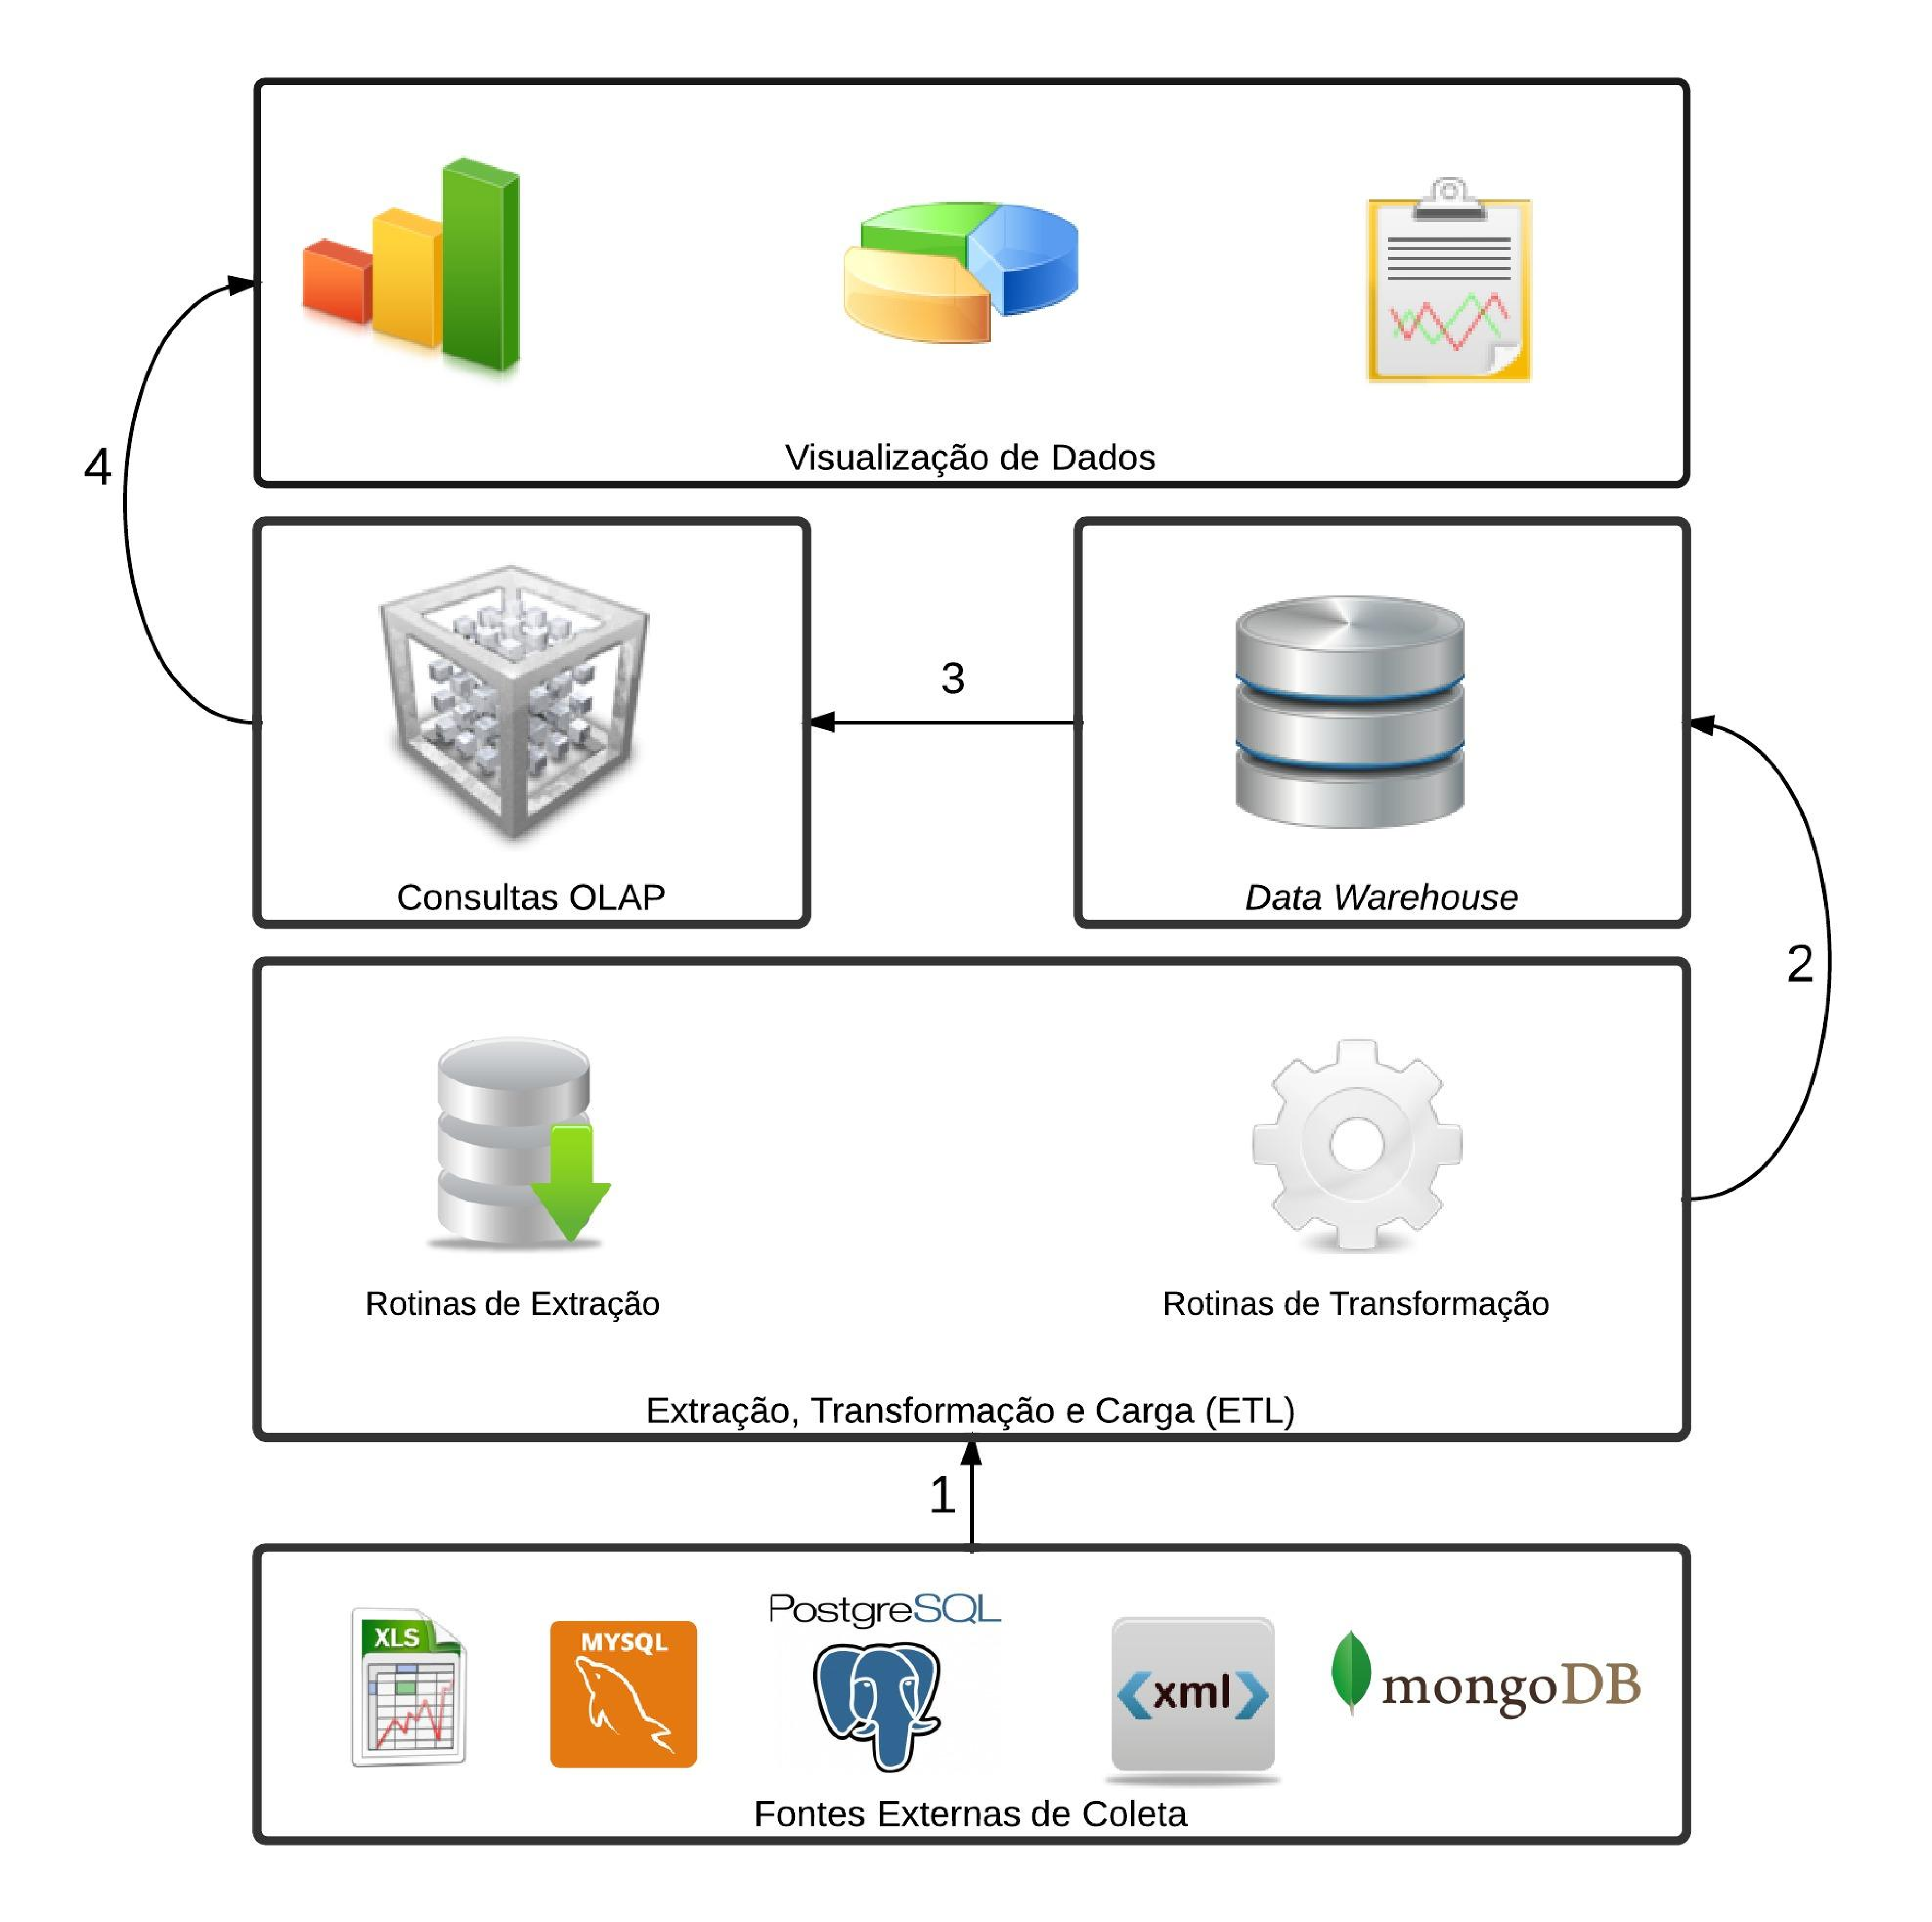
\includegraphics[keepaspectratio=false,scale=0.14]{figuras/Dwing.eps}
\caption{Arquitetura do Ambiente de \textit{Data Warehousing}}
\label{arquitetura}
\end{figure}
\FloatBarrier


Na Figura \ref{arquitetura}, as setas 1 e 2 representam o processo de \textit{Extraction-Transformation-Load (ETL)} que é o processo de extração, transformação e carga dos dados de forma automática e não intrusiva ao ambiente de desenvolvimento. Este processo pode consumir até 85\% de todo o esforço em um ambiente de \textit{Data Warehousing} \cite{Kimball2002}; A seta 3 representa as consultas \textit{On-Line Analytical Processing (OLAP)} que são operações de consulta e análise realizadas sobre \textit{data warehouse}projetado sobre um modelo dimensional \cite{Kimball2002} \cite{Codd1993}; A seta 4 representa a visualização dos dados em forma de gráficos, tabelas ou painéis customizáveis conhecidos como \textit{dashboards}.


A implementação do ambiente de \textit{data warehousing} mostrado na figura \ref{arquitetura} se deu pela ferramenta Analizo\footnote{Disponível em \url{http:/http://analizo.org/}}, responsável por coletar as métricas de código-fonte, a suite Pentaho BI Community\footnote{Disponível em \url{http://community.pentaho.com/}}, que dispõe de ferramentas de ETL e OLAP, um banco de dados MariaDB\footnote{Disponível em \url{http://mariadb.org/}} modelado sobre um modelo dimensional e o plugin Saiku Analitics\footnote{Disponível em \url{http://meteorite.bi/saiku}} para visualização de dados. 
% Seção do Estudo de Caso
\section {Estudo de Caso}

Visando a validação da solução apresentada na Seção \ref{sec:solucao}, foram consultadas as instituições citadas pelo Acórdão no 2314/2013 \cite{TCU:2013}. Dentre elas, o Instituto do Patrimônio Histórico e Artístico Nacional (IPHAN) que é autarquia da administração pública federal responsável pela gestão de diversos processos de preservação do patrimônio cultural, permitiu o acesso ao processo, documentos e o código-fonte Sistema Integrado de Gestão do Conhecimento (SICG), um dos primeiros softwares desenvolvidos sob um contrato de terceirização de serviços com a utilização de metodologias ágeis.

O Sistema Integrado de Gestão do Conhecimento (SICG) teve como objetivo automatizar o processo de trabalho decorrente da metodologia de inventário, cadastro, normatização, fiscalização, planejamento e análise e gestão do patrimônio material. Esta solução de software foi construído na linguagem Java com a utilização de\textit{frameworks} como VRaptor e Hibernate, durante 24 \textit{releases} mensais.

\subsection{Protocolo do Estudo de Caso}
Seguindo a metodologia proposta por Wohlin \cite{wohlin2012experimentation}, foi construído um protocolo de estudo de caso que foi baseado em Brereton \cite{brereton2008using} quanto aos aspectos gerais e Yin \cite{yin2011applications} com relação as ameaças à validade do estudo. 

O objeto do estudo de caso é a avaliação em ambiente de \textit{data warehousing} a detecção dos cenários de Limpeza de código-fonte e o comportamento taxa de aproveitamento de oportunidades de melhoria de código-fonte de forma que o processo de medição da qualidade do código-fonte possa servir como um critério de aceitação do produto por parte do fiscal do técnico do contrato de terceirização do produto de desnvolvimento de software. A fonte de coleta dos dados, para este estudo de caso, é o código-Fonte do Sistema Integrado de Gestão do Conhecimento.

Com relação as ameaças citadas por Yin, a validade de construção pôde ser obtida com utilização da abordagem GQM para selecionar indicadores que represetem a realide conhecida. Com relação a validade interna do estudo está garantida quando se consegue observar as relações causais e todos os elementos que as compõem. No presente estudo de caso, a taxa de aproveitamento de oportunidades de refatoração é diretamente dependente da quantidade de cenários de limpeza identificados desde que o número de classes permaneça o mesmo. Quanto a validade externa, destaca-se que a utilização de um estudo de caso não é suficiente para generalizar os resultados dele obtidos, sendo necessário a utilização de estudo em múltiplos casos, a fim de comprovar resultados genéricos \cite{yin2011applications}. Com relação a confiabilidade, a partir da documentação da implementação do ambiente de \textit{Data Warehousing} conjuntamente com o protocolo de estudo de caso e as bases de dados das métricas de código-fonte, garante-se a repetição do estudo de caso e por conseguinte a confiabilidade.

\subsection{Execução e Resultados do Estudo de Caso}
\label{sec:resultados}
Para analisar os cenários de limpeza de código-fonte, foram extraídas as métricas de código-fonte de cada classe e analisadas conforme a Tabela \ref{tab:cenarios}. Para cada \textit{release}, foram identificados, conforme a Figura \ref{fig:cenarios-release}, os cenários de limpeza de código-fonte. Para se mostrar maior nível de detalhes dos cenários de limpeza de código-fonte, realizou-se uma consulta OLAP de \textit{Drill-Down}, que tem objetivo de expor mais detalhes na visualização dos dados \cite{Kimball2002}, sobre o modelo dimensional do \textit{data warehouse}. 


\begin{figure}[ht!]
\centering
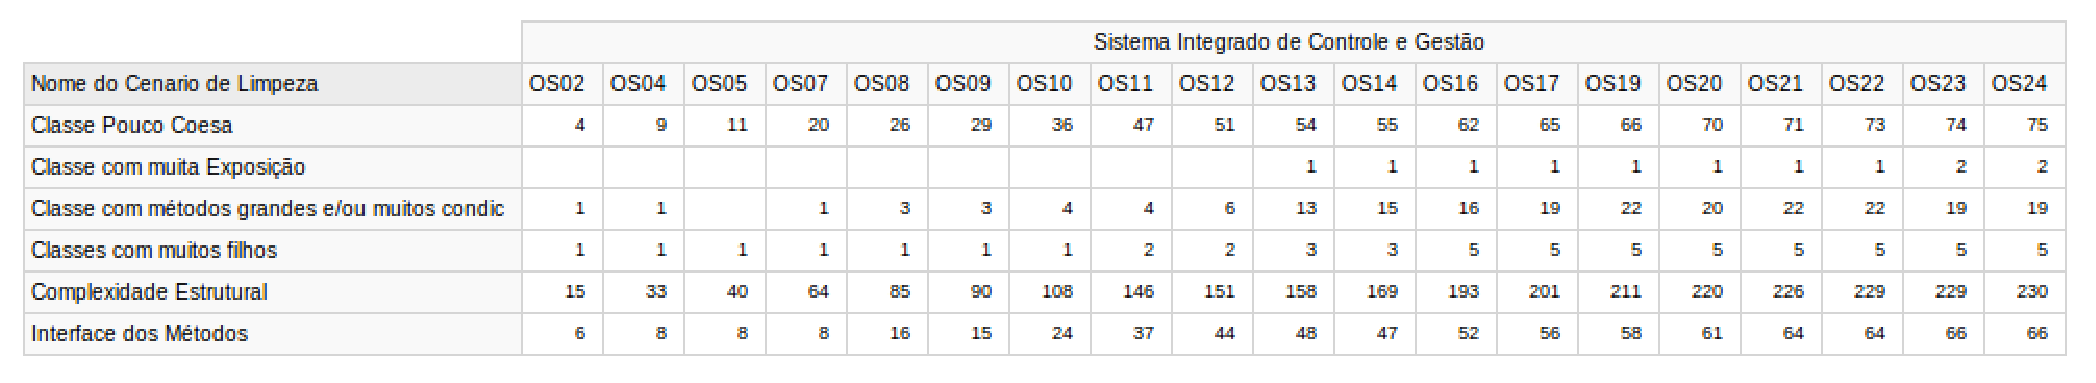
\includegraphics[keepaspectratio=true,scale=0.43]{figuras/total-cenario-tipo.eps}
\caption{Total de Cenários de Limpeza de Código-Fonte identificados por cenário e \textit{Release}}
\label{fig:cenarios-release}
\end{figure}
\FloatBarrier

A fim de se obter o número total de cenários de limpeza por cada uma das releases de software analisadas, como se observa na Figura \ref{fig:cenarios-total}, foi realizada uma consulta OLAP de \textit{Drill-Up}, que tem o objetivo de agregar o nível de visualização dos dados \cite{Kimball2002}, sobre os dados obtidos na Figura \ref{fig:cenarios-release}.

\begin{figure}[ht!]
\centering

\includegraphics[keepaspectratio=true,scale=0.45]{figuras/total-cenarios-release.eps}
\caption{Total de Cenários de Limpeza de Código-Fonte por Release}
\label{fig:cenarios-total}
\end{figure}
\FloatBarrier

Conforme é possível observar nas Figuras \ref{fig:cenarios-release} e \ref{fig:cenarios-total}, foram detectados mais cenários de limpeza de código-fonte dos tipos \textbf{Complexidade Estrutural}, que corresponde entre 55\% a 68\% da quantidade total de cenários identificados; \textbf{Classe Pouco Coesa} e \textbf{Interface dos Métodos} respectivamente. Os três Cenários de Limpeza com menor número de incidências foram \textbf{Classe com Muita Exposição}, \textbf{Classe com Muitos Filhos} e \textbf{Classe com Métodos Muito Grande e/ou com muitos condicionais}.

Considerando que é importante conhecer as classes com maior incidência de problemas com relação limpeza de código-fonte, foram identificadas, como se mostra na Figura \ref{fig:worst-10-cenarios}, as 10 classes que apresentaram a maior quantidade de cenários de limpeza de código-fonte. Para se obter a informação desta consulta foram necessárias uma consulta OLAP de \textit{Drill Down} sobre algumas dimensões e outra de \textit{Slice and Dice}, que tem o objetivo de selecionar os dados, sobre o resultado a consulta de \textit{Drill-Down}.    

\begin{figure}[ht!]
\centering
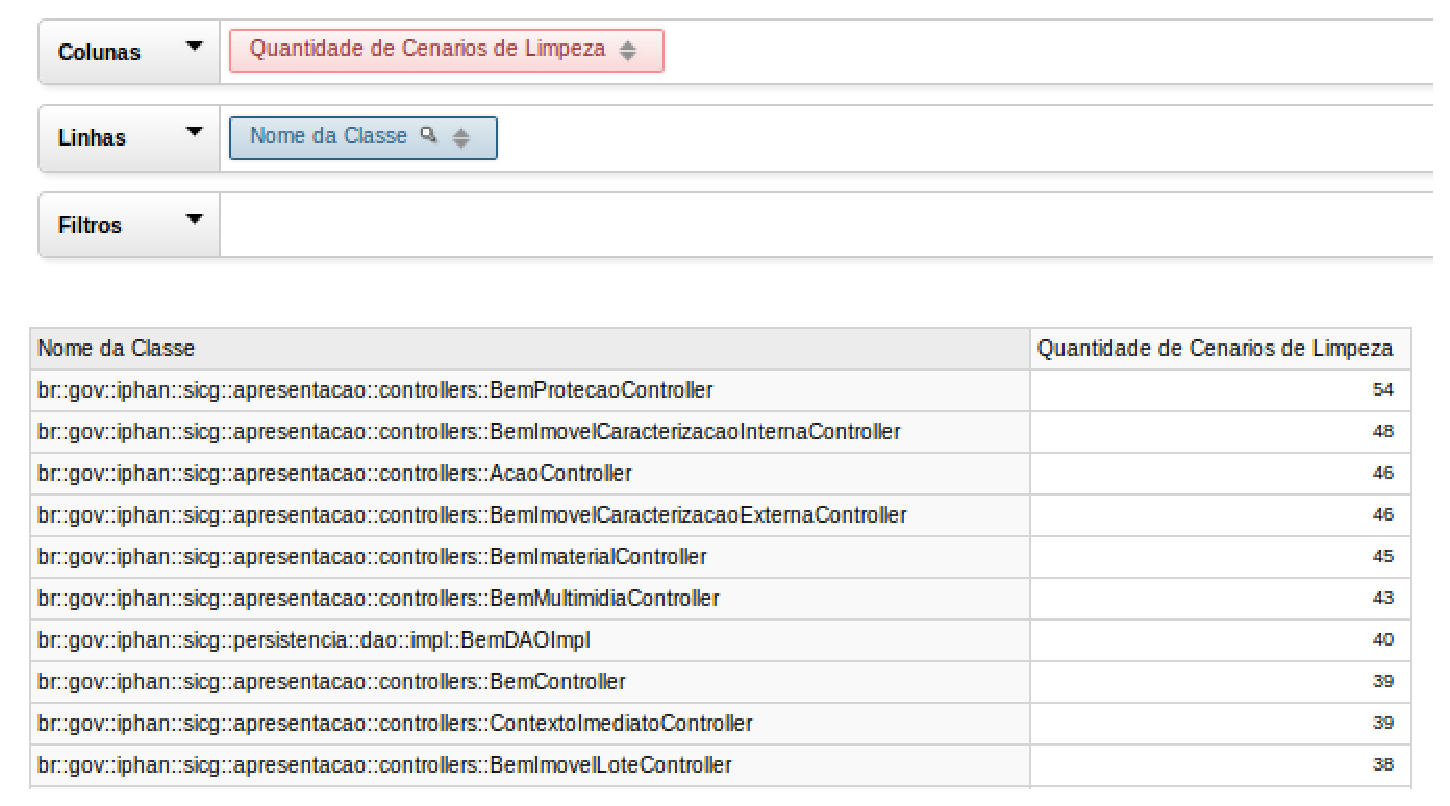
\includegraphics[keepaspectratio=true,scale=0.55]{figuras/10-best.eps}
\caption{As 10 classes com maior número identificado de Cénarios de Limpeza}
\label{fig:worst-10-cenarios}
\end{figure}
\FloatBarrier

Com a quantidade de classes e o total de cenários de limpeza de código-fonte, foi possível calcular a Taxa de Aproveitamento de Oportunidade de Melhoria de Código-Fonte por cada release do software conforme se mostra na Figura \ref{fig:taxa-cenarios}.

\begin{figure}[H]
\centering
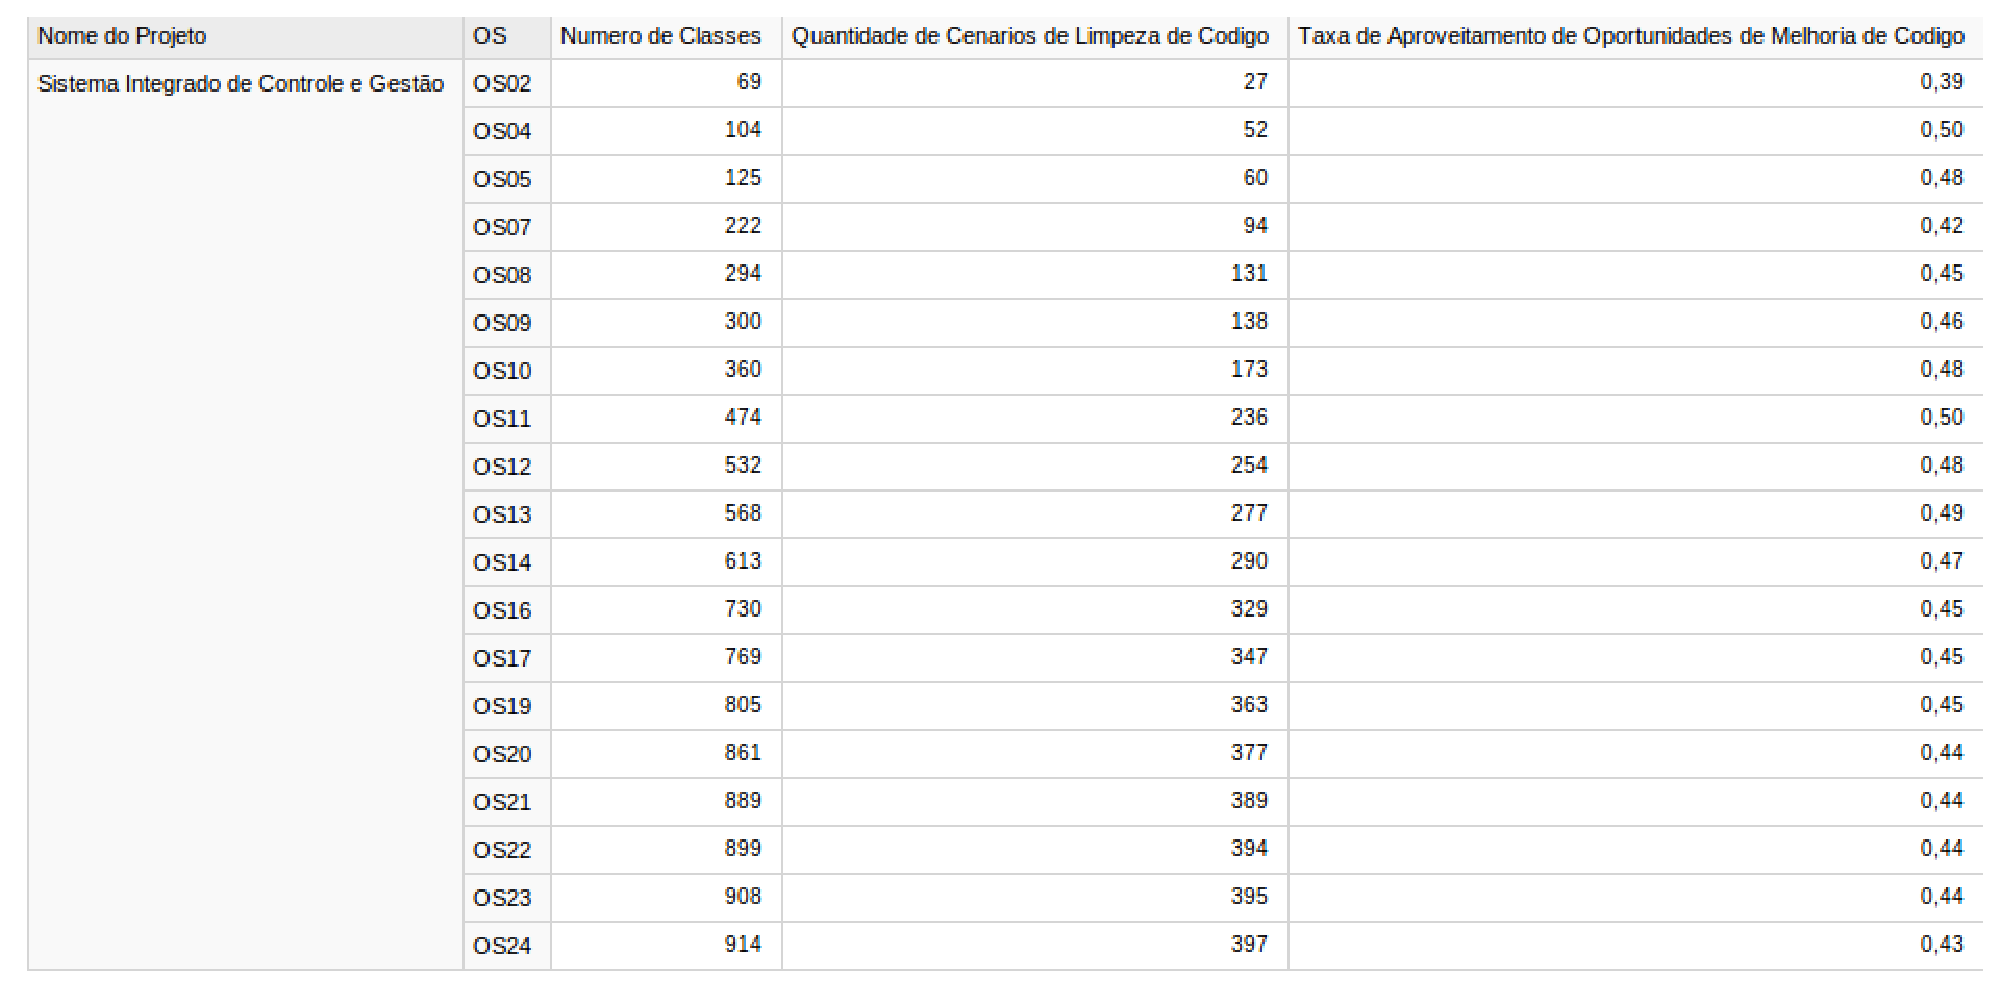
\includegraphics[keepaspectratio=true,scale=0.38]{figuras/taxa-parcial.eps}
\caption{Taxa de Aproveitamento de Oportunidades de Melhoria de Código-Fonte}
\label{fig:taxa-cenarios}
\end{figure}
\FloatBarrier

Observa-se, por meio da Figura \ref{fig:taxa-cenarios}, que o valor da Taxa de Aproveitamento de Oportunidade de Melhoria de Código-Fonte possui uma tendência entre 0,4 a 0,5. Este fato pode indicar duas hipóteses: a primeira de que o projeto cresceu em uma taxa muito maior que a quantidade de cenários de limpeza, indicando assim uma estabilidade na complexidade do projeto; ou que não foram promovidas atividades de melhoria de código-fonte ao longo das 24 releases.

% Seção de Conclusão e Trabalhos Futuros
\section{Conclusões e Trabalhos Futuros}

No início deste trabalho, elaborou-se a seguinte questão de pesquisa: \textbf{Como incorporar, do ponto de vista do fiscal técnico do contrato, a qualidade do código-fonte como critério de aceitabilidade do produto?}. A partir desta questão, foram elaboradas algumas questões específicas e métricas específicas utilizando o GQM \cite{Basili96b}.

Considerando o objetivo de automatizar o processo de medição da qualidade interna do produto de software (objetivo específico OE1) como divisor entre incorporação da qualidade do código-fonte como critério de aceitação do produto, acredita-se que o ambiente de \textit{data warehousing} pode configurar uma boa solução para automatizar a medição de qualidade do código-fonte, pois foram automatizados desde a extração das métricas de código-fonte, a interpretação dos cenários de limpeza de código-fonte, o cálculo da taxa de aproveitamento das oportunidades de melhoria do código-fonte até a exibição dos dados em tabelas e gráficos.

Com os resultados apresentados na Seção \ref{sec:resultados}, verifica-se que uma outra contribuição ambiente de \textit{data warehousing} foi alcançada por meio das consultas OLAP que permitiram flexibilidade necessária para se avaliar tanto em nível de projeto (objetivo específico OE2), quanto em nível local (objetivo específico OE3) a saúde do projeto com relação a qualidade do código-fonte. Por meio de um ambiente de \textit{data warehousing} semelhante ao apresentado, os fiscais técnicos dos contratos podem contar com mecanismos rápidos de auditoria sobre a qualidade do código-fonte, de forma seja possível atribuir níveis de aceitação com relação a qualidade do código-fonte. 

Cabe ressaltar que o IPHAN não realizou análise das métricas de código-fonte e nem pediu a contratada que documentasse as atividades de refatoração de código-fonte ao longo da execução do contrato, logo não se pôde aprofundar nas investigações das duas hipóteses levantadas (na Seção \ref{sec:resultados}) com relação ao comportamento da taxa de aproveitamento de oportunidades de melhoria do código-fonte (objetivo OE4). Como trabalho futuro, recomenda-se que essa investigação das hipóteses seja feita nos órgãos citados pelo Acórdão no 2314/2013 \cite{TCU:2013}, em que seja possível acompanhar as atividades de refatoração do código-fonte ao longo do desenvolvimento de software.





\bibliographystyle{sbc}
\scalefont{.9}
\bibliography{myReferences}
\end{document}

